\chapter{Applicability to Amputee Data}
\label{chp:amputee-data}

The collection of labelled training data is ardours, this becomes more acute when the subject has restricted movement such as for an amputee. Therefore any system which can reduce the data requirements for these individuals is of benefit. In Chapter \ref{chp:personalisation} methods for personalisation of a machine learning model using additional data from other subjects were demonstrated to both improve the performance of a model and reduce the data requirements for that model. Within this chapter these methods will be implemented for an amputee to investigate it they are applicable to someone with a substantially different gait to the normal population.

Within this chapter we will investigate whether the personalisation methods developed in Chapter \ref{chp:personalisation} can use prior non-amputee data to improve the performance of an \acrshort{lmr} classifier for an individual amputee.

The contributions of this Chapter are:
\begin{itemize}
    \item Collection of amputee gait data that is directly comparable to non-amputee data
    \item Comparison of shank \acrshort{imu} data between non-amputee, intact limb and prosthetic
    \item Demonstration of performance differences of \acrshort{lmr} network of intact and prosthetic side
    \item Demonstration of transfer learning from non-amputee data to an amputee for \acrshort{marg} gait data
\end{itemize}

% Sometimes an overview of the chapter
First related works are presented. This is followed by Section \ref{sec:amputee-methods} in which an explanation of the methods used and presentation of amputee data collected are provided. Following this the results of a baseline model performance, and performance of two personalisation methods in Sections \ref{sec:amputee-baseline}, \ref{sec:amputee-supplementation} and \ref{sec:amputee-transfer} respectively. Finally discussion and conclusion are given in Sections \ref{sec:amputee-discussion} and \ref{sec:amputee-conclusions}.


%-----------------------------------------------------------------
\section{Related Works}
\label{sec:amputee-related-works}
The gait of a lower-limb amputee varies dramatically between individuals\cite{Lonini2016} often presenting asymmetrically\cite{Roerdink2012}. This asymmetry is seen in many gait features including stance and swing periods, and hip, knee and ankle joint moments\cite{Adamczyk2015, Harandi2020}. A common explanation for this is the reduced push-off capacity of the prosthetic leg, but it may also be due to discomfort of the prosthetic\cite{Hak2014}. Many lower limb amputees attempt to maximise the capacities of their intact limb to counteract the limitations of their prosthetic device\cite{Ochoa-Diaz2020}. This asymmetry results is a substantially different gait from the norm. Therefore techniques that work for non-amputees are not necessarily directly applicable to amputees or other gait impairments\cite{Jamieson2021}.

Lonini et al considered a personal model trained from a target's data was required. Or if a global model from other patients was all that was required. The study involved the classification of physical activities based on sensor data from a waist worn accelerometer.  Eleven non-amputee and ten patients who use an Knee-Ankle-Foot Orthotic (KAFO) device were asked to perform five actions. There work suggested that models trained exclusively of subject without gait impairments performed poorly when tested using the KAFO subjects. However the model trained from only KAFO subjects performed only slightly worse than the personalised baseline.\cite{Lonini2016}

Jamieson et al performed a study comparing the performance of supervised classifiers for both amputee and non-amputee carrying out the same activities. Data collected was collected from a hip mounted \acrshort{imu} with participants asked to walk an improvised route in the vicinity of their homes. A both \acrfull{svm} and \acrshort{lstm} networks were trained to classify different locomotive activities. Classifiers were trained with varying sets of data constructed by \acrfull{looxv}. Several configurations of subjects were tested. Most notable a network was trained using exclusively non-amputee data but tested using amputees data. Classification accuracy fell $~78\%$ for non-amputees to an average of $~55\%$ for the four amputees. Jamieson concluded that classifiers trained using exclusive persons without gait impairments would not be suitable for those with impaired gait.\cite{Jamieson2021}

Gao et al presented work investigating Reinforcement Learning (RL) schemes for controlling a lower limb prosthesis that was personalised to an individual. They first collected data from two non-amputees wearing a below knee prosthetic device. This data was used to generate base knowledge that could be used as a starting point for their RL scheme. Using the human locomotive simulator OpenSim they implemented models of amputee gaits. These were then use to demonstrate a RL scheme that could adapt to an individual.\cite{Gao2020a}

There is very limited literature on applying classifiers from non-amputees subjects to those with amputations. The literature that exists suggest that in order to achieve adequate classification accuracy the gait abnormalities of an amputee must be taken into account

From the literature surveyed the following gaps were identified:
\begin{itemize}
    \item No work has attempted to use transfer learning to personalise a non-amputee \acrshort{lmr} model for an amputee
    \item No papers have investigated the difference in classification performance between amputated and in-tact limb
\end{itemize}

The remainder of this chapter will focus on investigating these gaps.

%-----------------------------------------------------------------
\section{Methods and Materials}
\label{sec:amputee-methods}
% Recap methods and what has changed
The methods used in this chapter will mirror those used in previous chapters. Additional data for an amputee was collected. This was used to generate a new set of baselines to compare the results of the personalisation methods previously developed against.

Data was collected from a single left trans-tibial amputee wearing a Blatchford Echelon VT prosthetic limb. The data was collected by Blatchford Product Limited. The data was collected in the same manner as previously described, however a clinician at the centre held the phone and annotated the activities in order to reduce the risk of fall. Table \ref{tab:summary-of-episode-amputee-data} shows a summary of the data collected including the number of data samples and the number of episode for each activity.

\begin{table}[hbt]
    \centering
    \caption{Summary of amputee gait data collected}
    \label{tab:summary-of-episode-amputee-data}
    \begin{tabularx}{\textwidth}{c *{6}{Y}}
        \noalign{\hrule height 1.5pt}
        \textbf{Activity} & WALK & \glsentryshort{ra} & \glsentryshort{rd} & \glsentryshort{sa} & \glsentryshort{sd} & STOP \\
        \hline
        \textbf{Samples} & 38114 & 6159 & 7194 & 2872 & 2450 & 11763 \\
        \textbf{Episodes} & 26 & 7 & 7 & 4 & 4 & 15 \\
        \noalign{\hrule height 1.5pt} \\
    \end{tabularx}
\end{table}

As significantly less data is available to test with, adjustments had to be made the quantities used in each of the sets. The test data set was reduced from 5000 windows to 250 windows. The range of training windows tested was reduced to between 100 and 750. Additionally in order to ensure that there was sufficient episodes for \acrshort{sa} and \acrshort{sd} each of the stair episodes was split up into new episodes containing a maximum of 200 samples each. This increased the number of available episode to episodes for both stair activities. 

Due to asymmetry the left and right ankle data cannot be combined. This will be described further in the following section. All other quantities and hyper-parameters remained the same.

\subsection{Amputee Gait Data}
Gait asymmetry of amputees means that unlike in the previous chapter the left and right ankle data cannot be combined to increase the dataset size. Instead both sides will be evaluated independently to investigate the performance differences between the side. Figure \ref{fig:ch6_amputee_gyro_trends} shows the angular velocity of the shank in the Saggital plane for the intact and prosthetic limbs of a left amputated trans-tibial amputee. The left ankle has been transformed using Equation \ref{eqn:left-right-transformation} so both ankles are presented in the same axes. For comparison the ankle angular velocity of the non-amputee subject 1 is shown.

% How does it differ from non-amputee gait data
\begin{figure}[p]
    \begin{tabular}{lccc}
        & \textbf{Non-Amputee} & \textbf{Amputee -- Intact Limb} & \textbf{Amputee -- Prosthetic} \vspace{0.2cm}\\

        \rotatebox{90}{\enspace\qquad \textbf{Walking}} &
        \begin{subfigure}[b]{0.275\textwidth}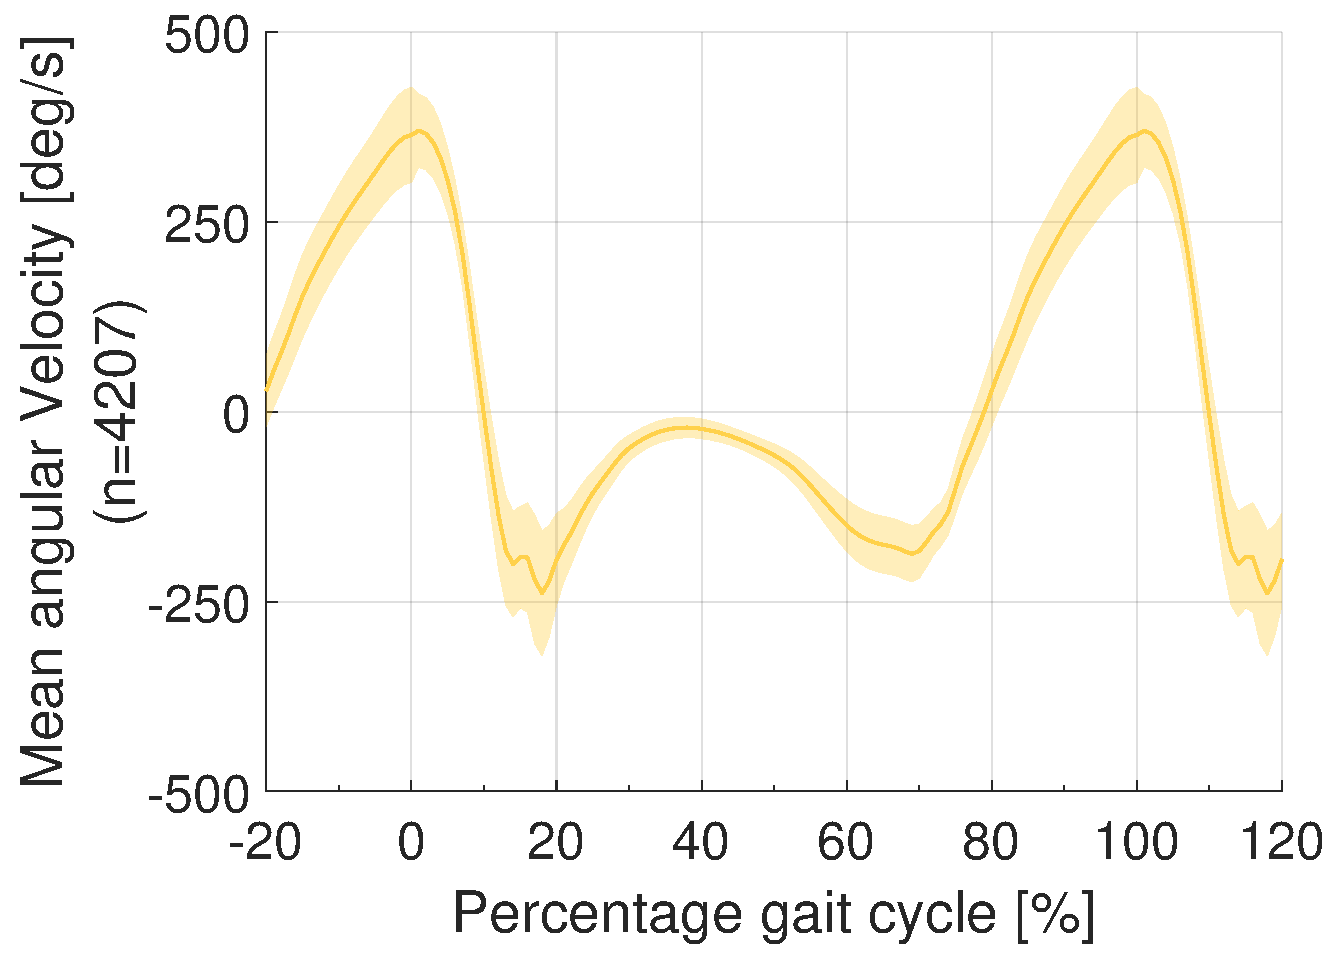
\includegraphics[width=\linewidth]{content/6-Amputee/Gait-Trends/ch6_subject_01_gait_trends_r_ankle_gyro_z_activity_walking.pdf}\end{subfigure} & \begin{subfigure}[b]{0.275\textwidth}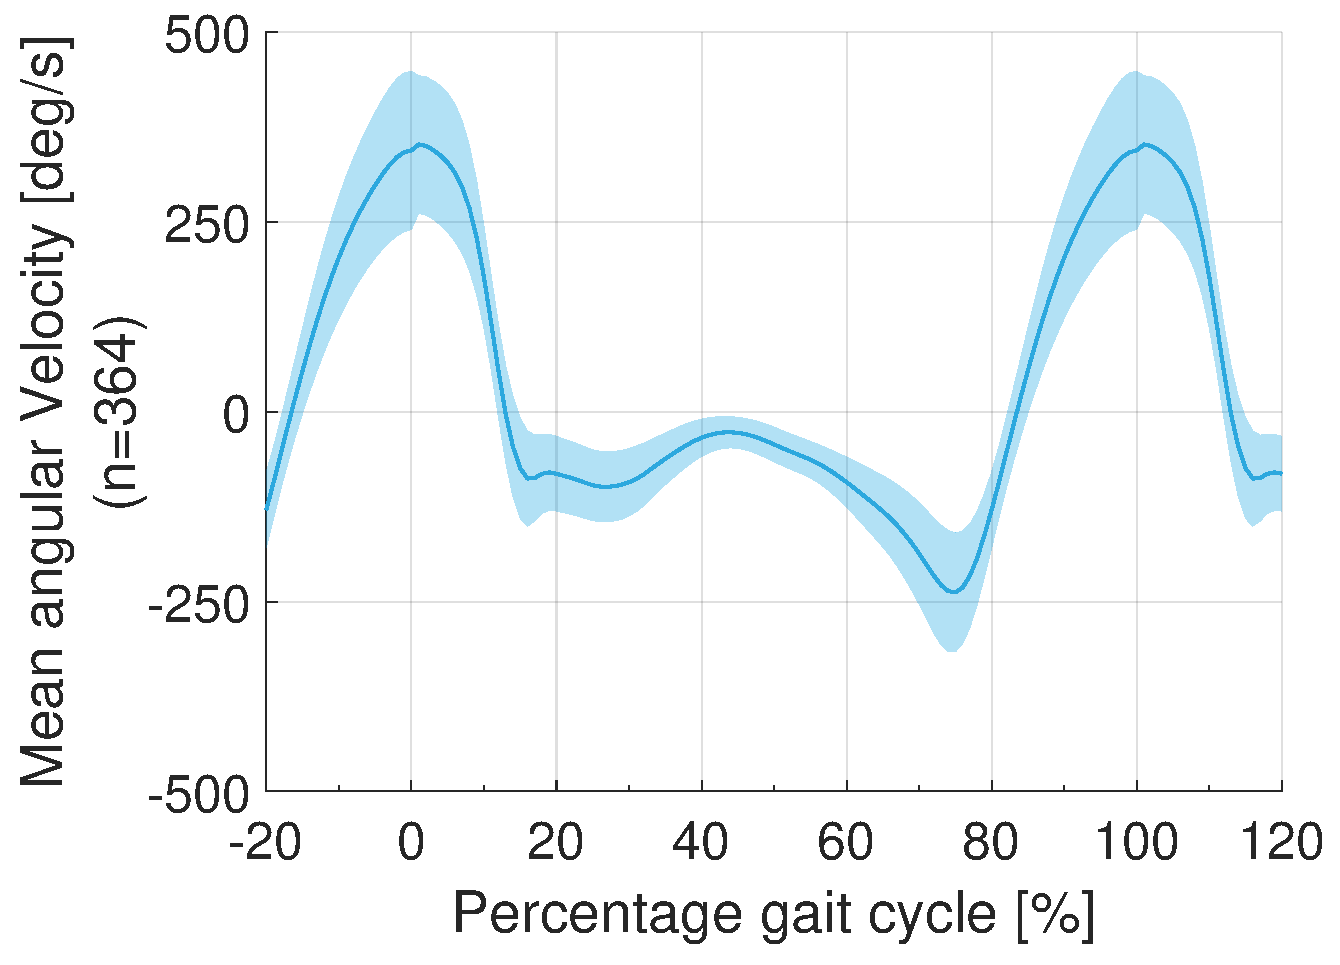
\includegraphics[width=\linewidth]{content/6-Amputee/Gait-Trends/ch6_amputee_gait_trends_l_ankle_gyro_z_activity_walking.pdf}\end{subfigure} &
        \begin{subfigure}[b]{0.275\textwidth}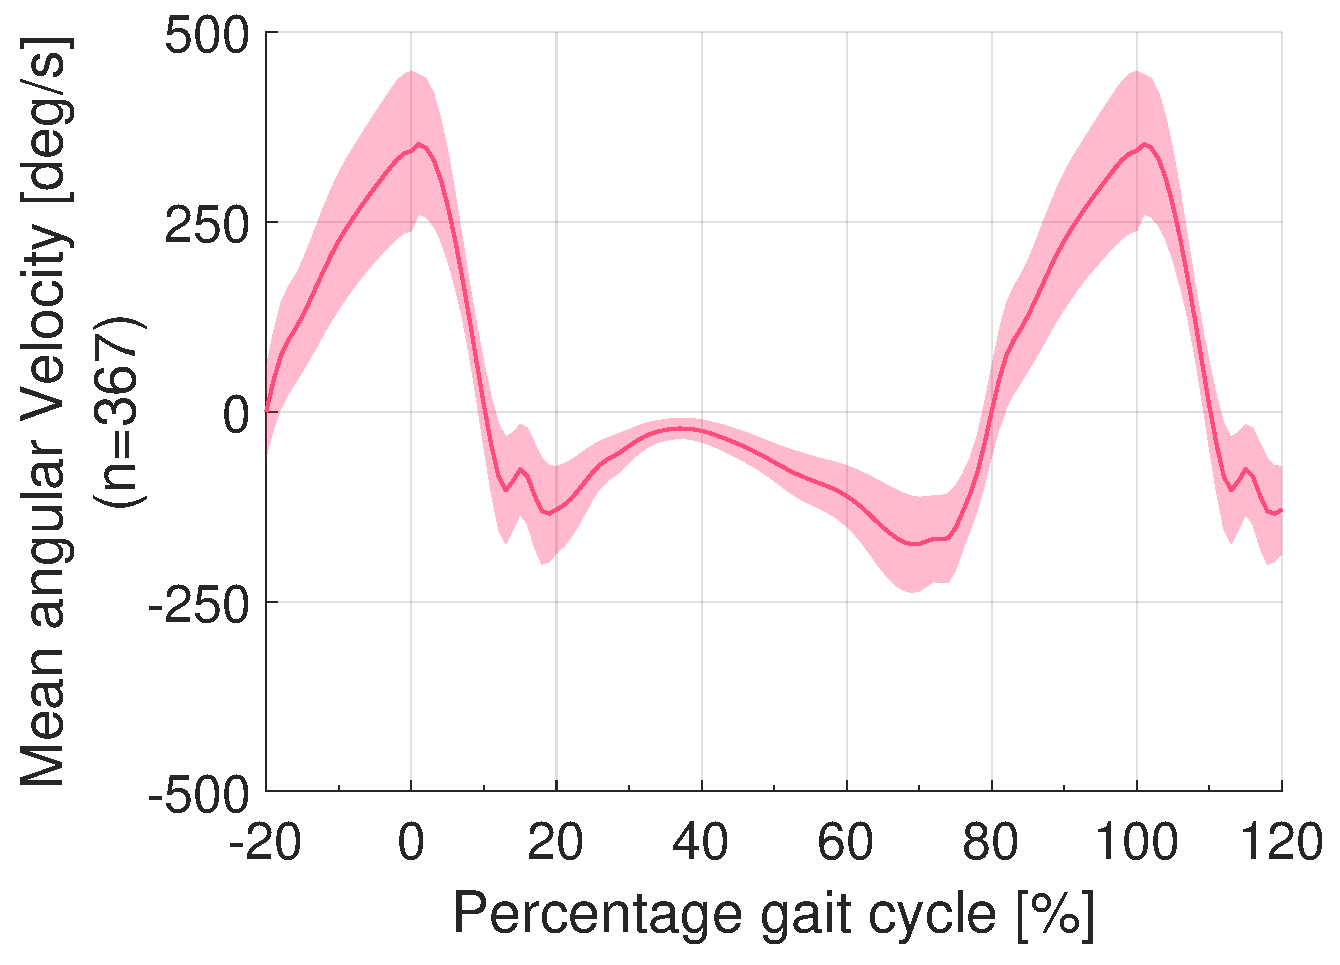
\includegraphics[width=\linewidth]{content/6-Amputee/Gait-Trends/ch6_amputee_gait_trends_r_ankle_gyro_z_activity_walking.pdf}\end{subfigure} \\
        
        \rotatebox{90}{~\quad \textbf{Ramp Ascent}} & 
        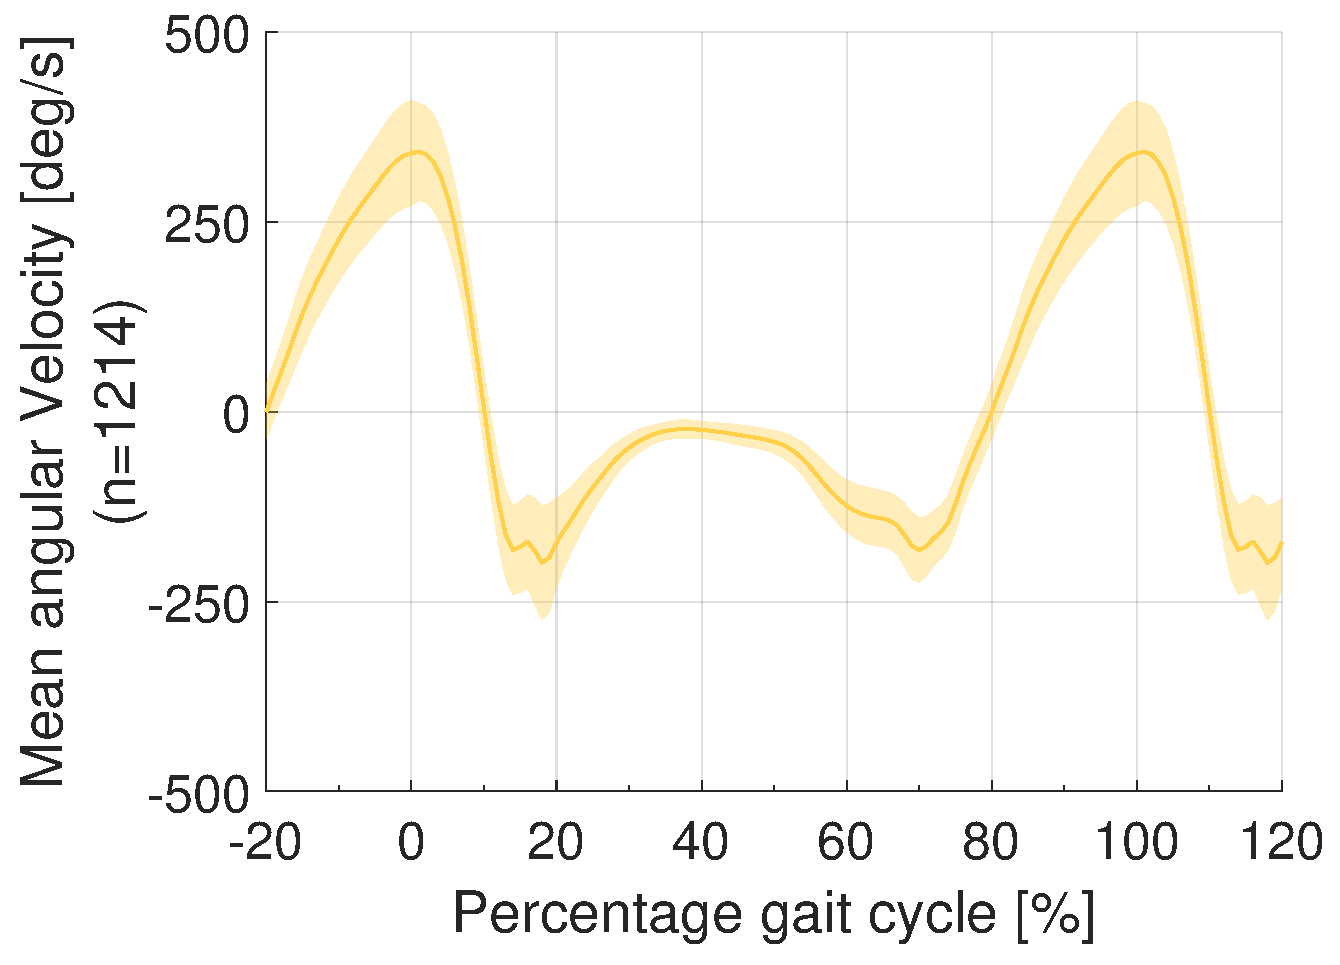
\includegraphics[width=0.275\linewidth]{content/6-Amputee/Gait-Trends/ch6_subject_01_gait_trends_r_ankle_gyro_z_activity_ramp_up.pdf} & 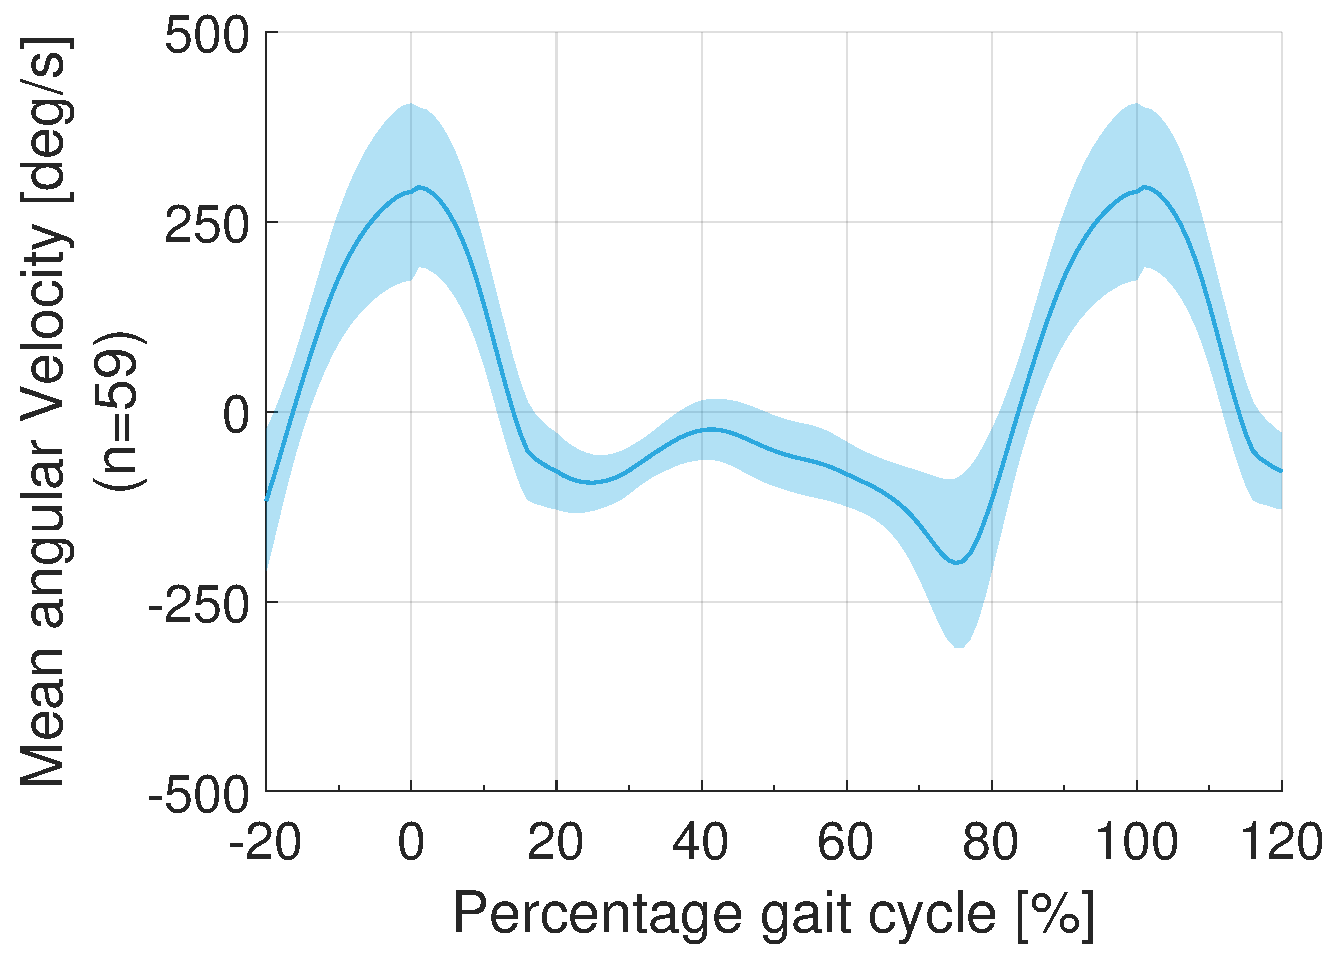
\includegraphics[width=0.275\linewidth]{content/6-Amputee/Gait-Trends/ch6_amputee_gait_trends_l_ankle_gyro_z_activity_ramp_up.pdf} &
        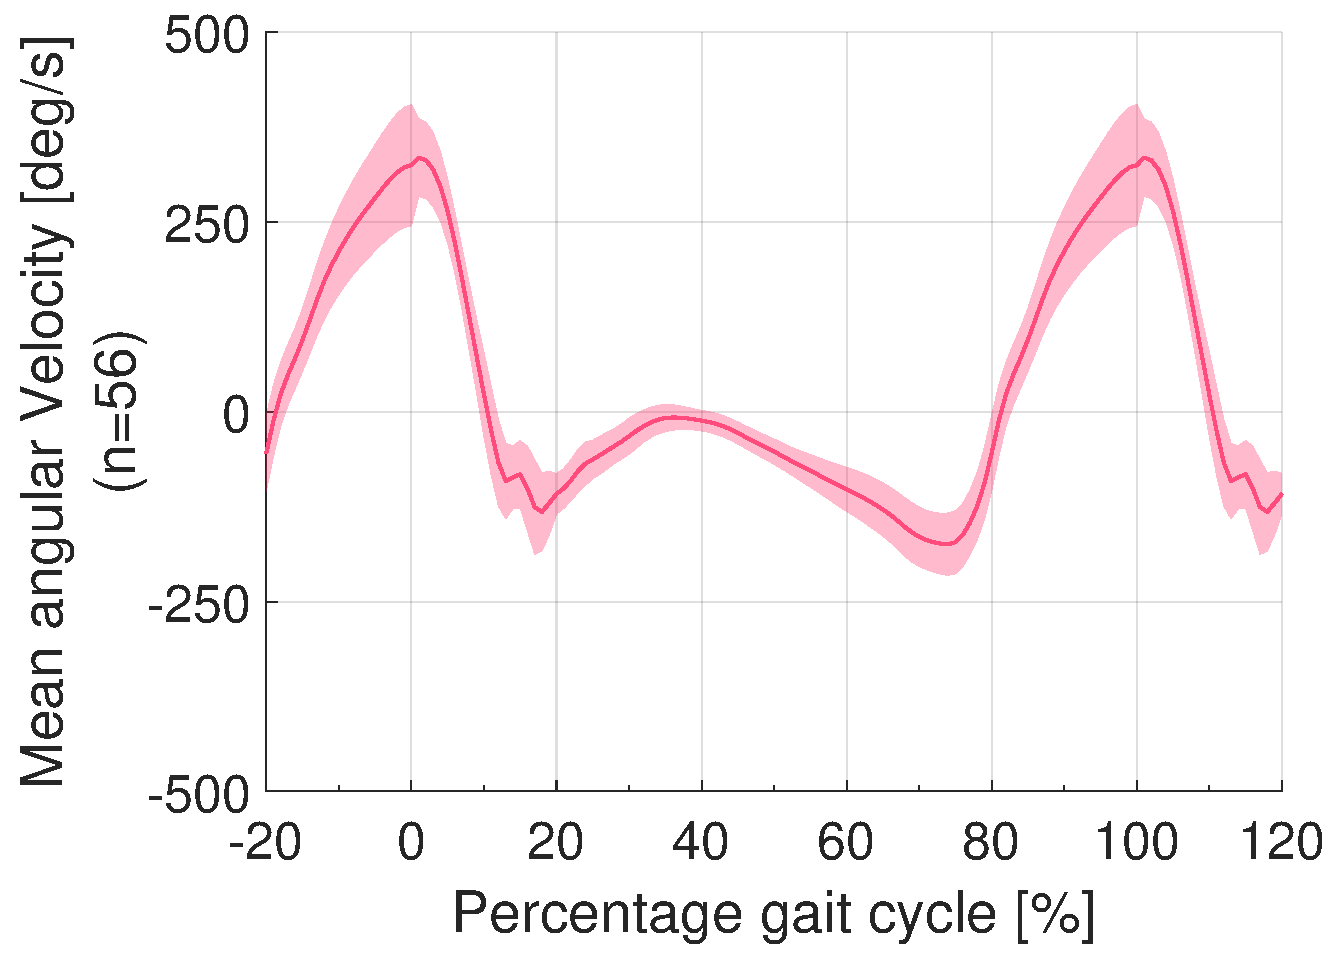
\includegraphics[width=0.275\linewidth]{content/6-Amputee/Gait-Trends/ch6_amputee_gait_trends_r_ankle_gyro_z_activity_ramp_up.pdf} \\
        
        \rotatebox{90}{\quad \textbf{Ramp Descent}} & 
        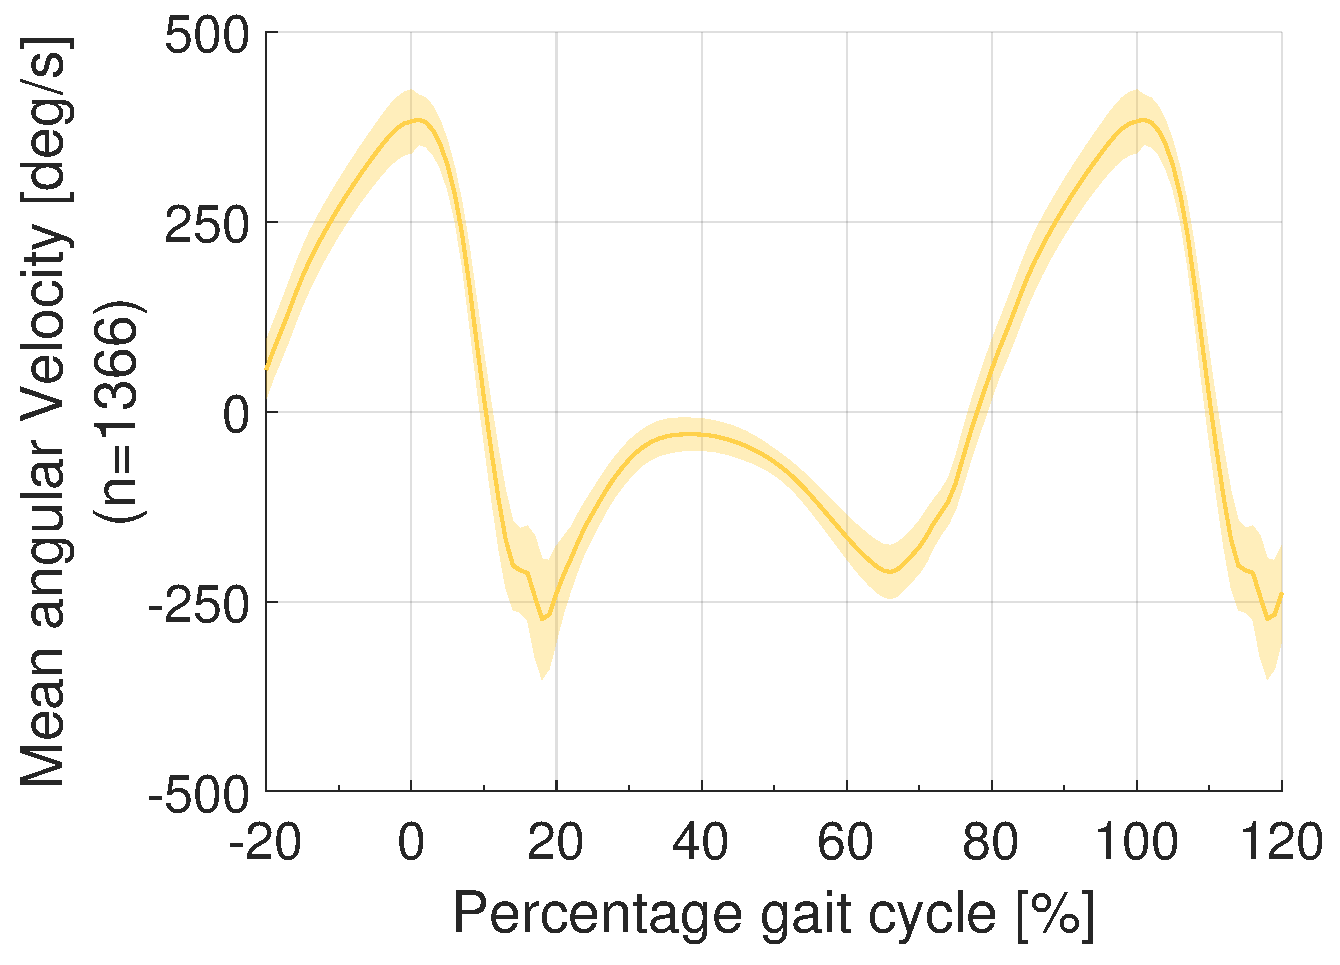
\includegraphics[width=0.275\linewidth]{content/6-Amputee/Gait-Trends/ch6_subject_01_gait_trends_r_ankle_gyro_z_activity_ramp_down.pdf} & 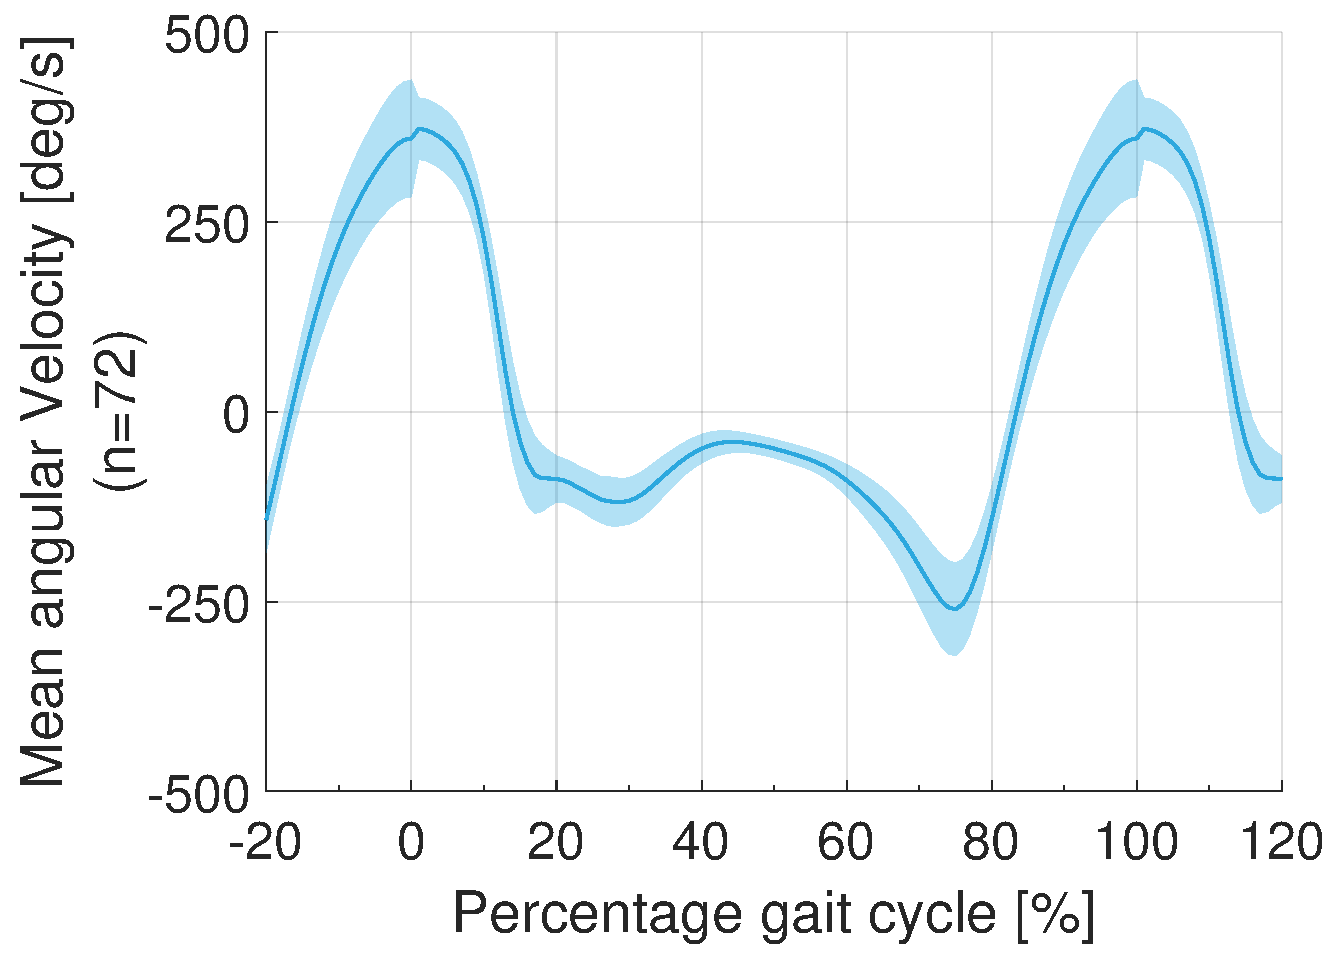
\includegraphics[width=0.275\linewidth]{content/6-Amputee/Gait-Trends/ch6_amputee_gait_trends_l_ankle_gyro_z_activity_ramp_down.pdf} &
        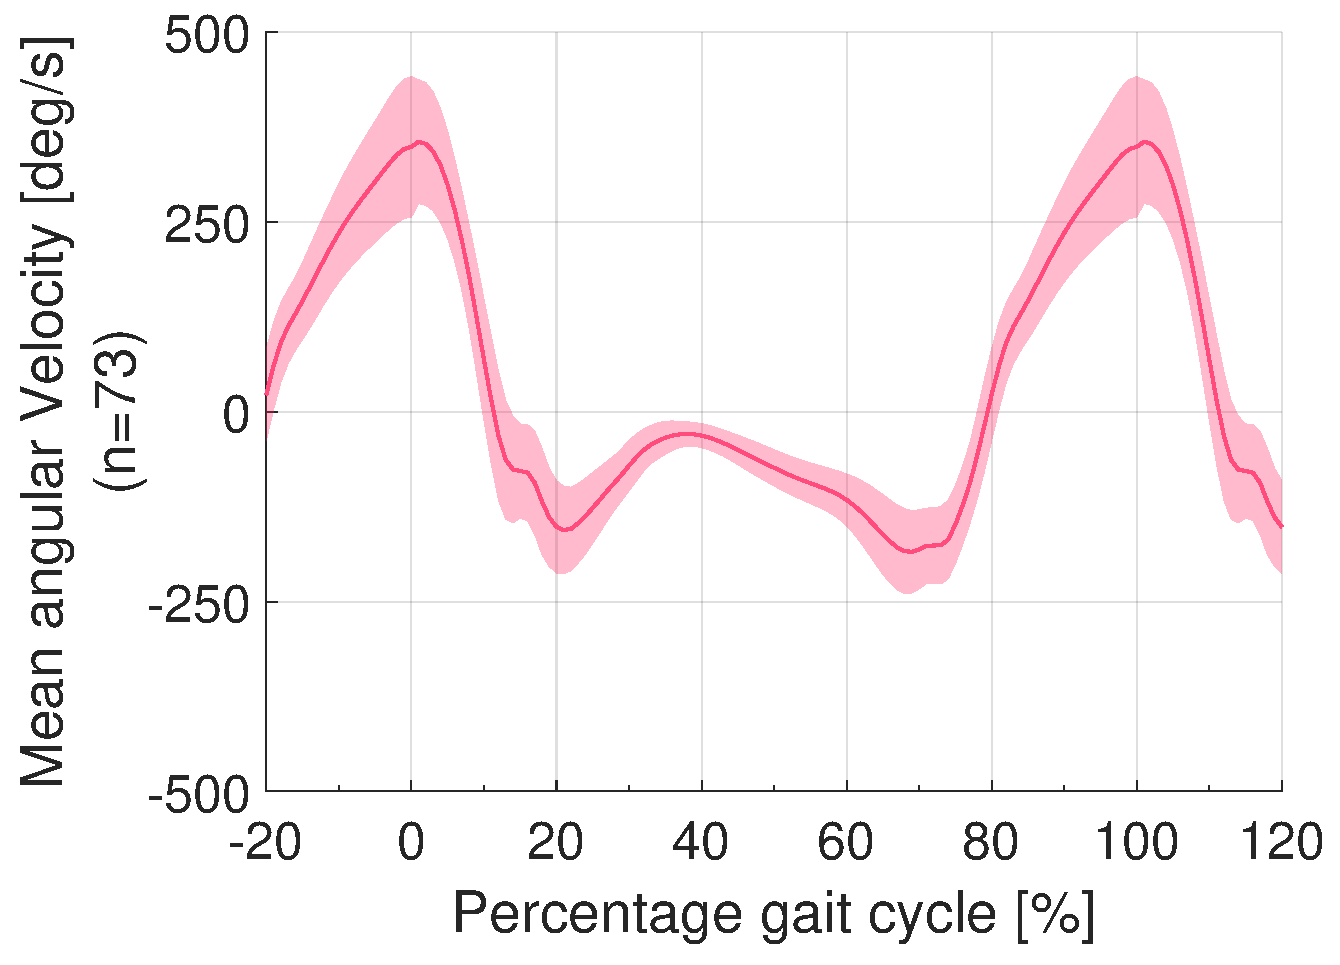
\includegraphics[width=0.275\linewidth]{content/6-Amputee/Gait-Trends/ch6_amputee_gait_trends_r_ankle_gyro_z_activity_ramp_down.pdf} \\
        
        \rotatebox{90}{~\quad \textbf{Stair Ascent}} & 
        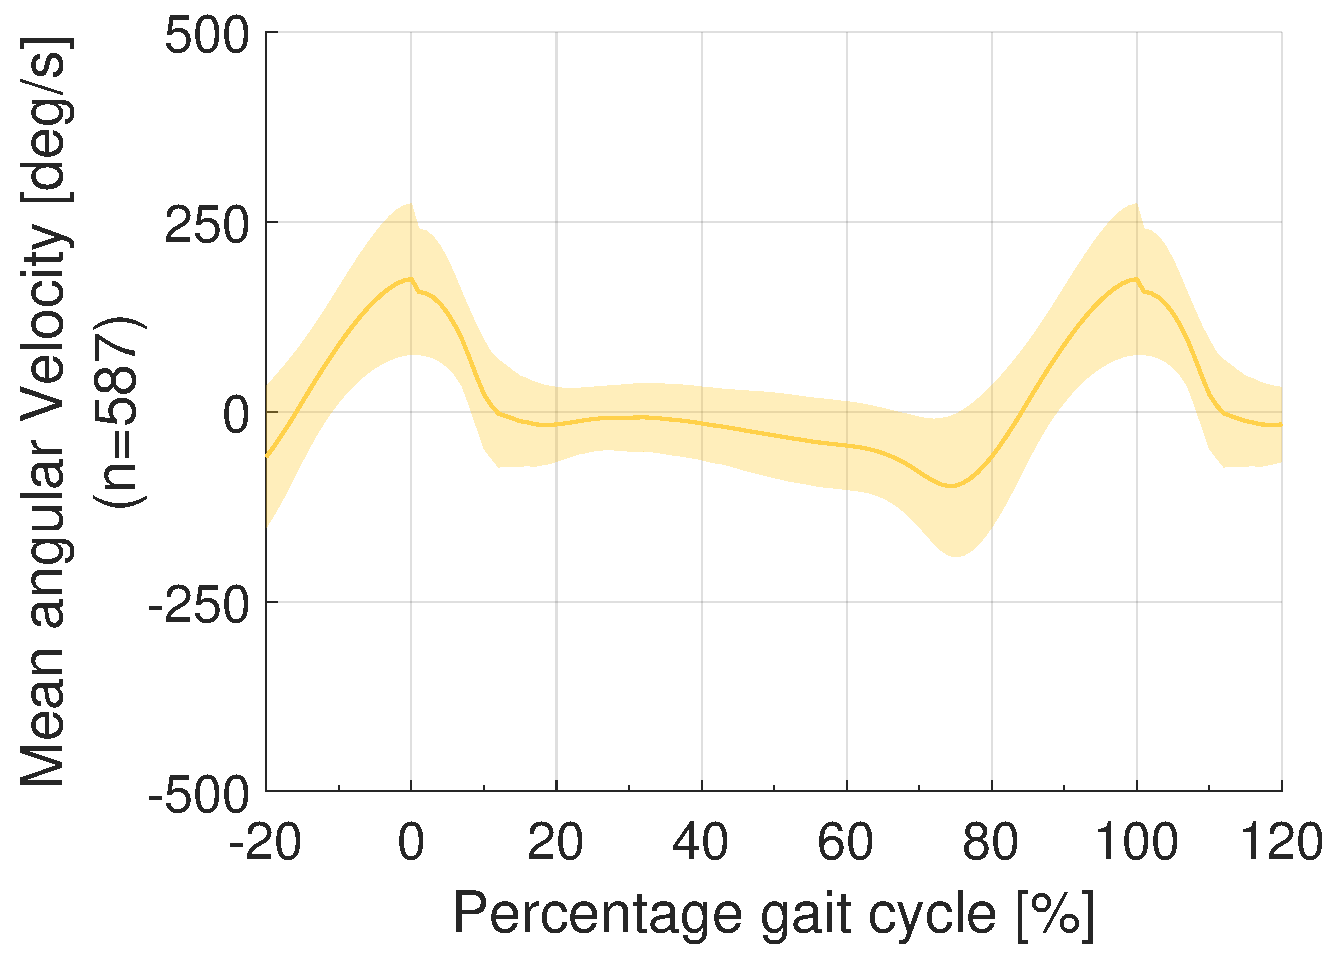
\includegraphics[width=0.275\linewidth]{content/6-Amputee/Gait-Trends/ch6_subject_01_gait_trends_r_ankle_gyro_z_activity_stair_up.pdf} & 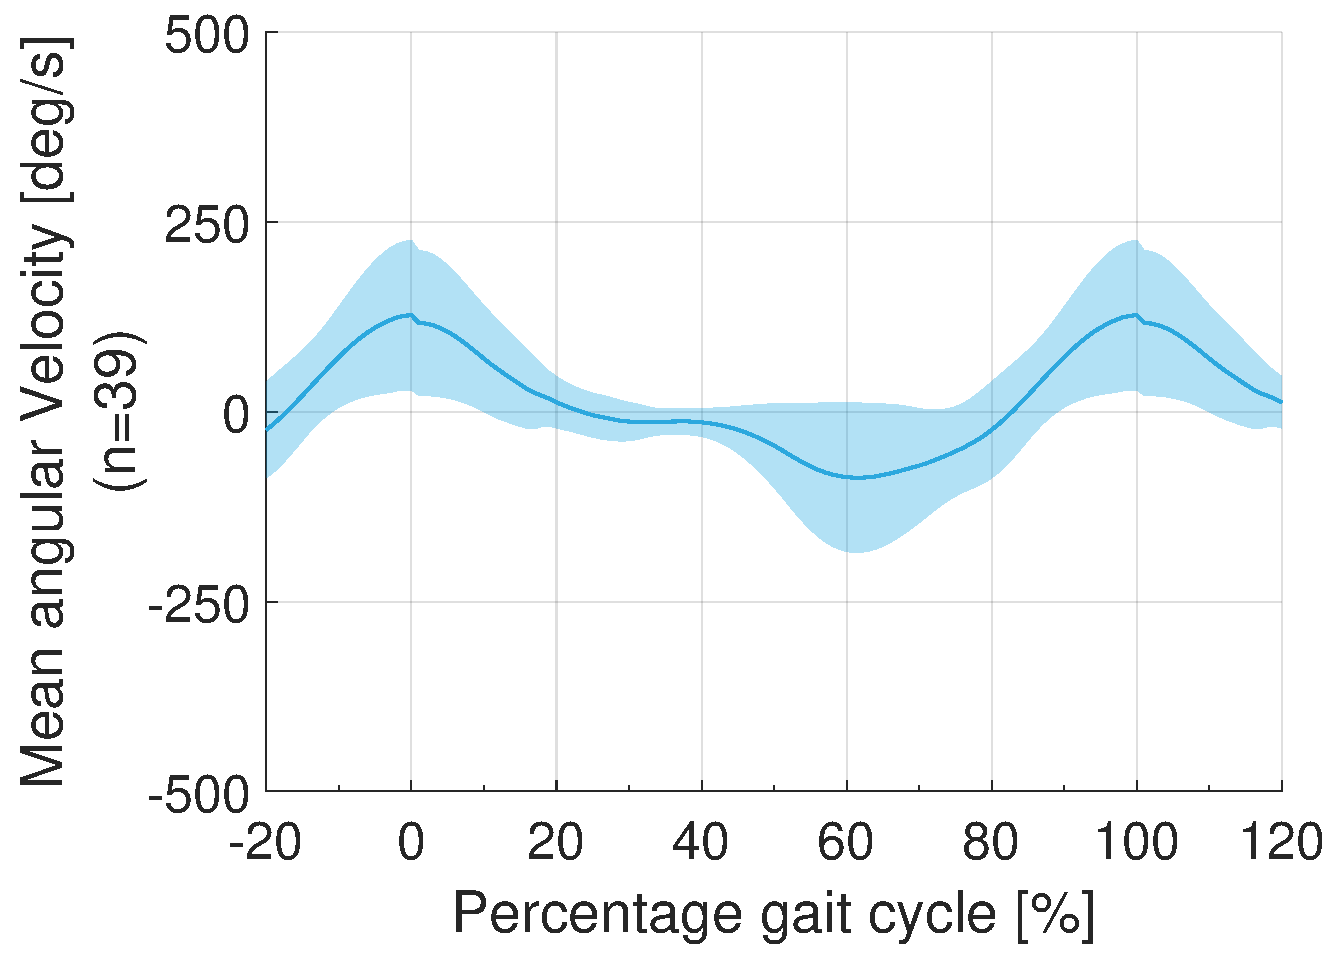
\includegraphics[width=0.275\linewidth]{content/6-Amputee/Gait-Trends/ch6_amputee_gait_trends_l_ankle_gyro_z_activity_stair_up.pdf} &
        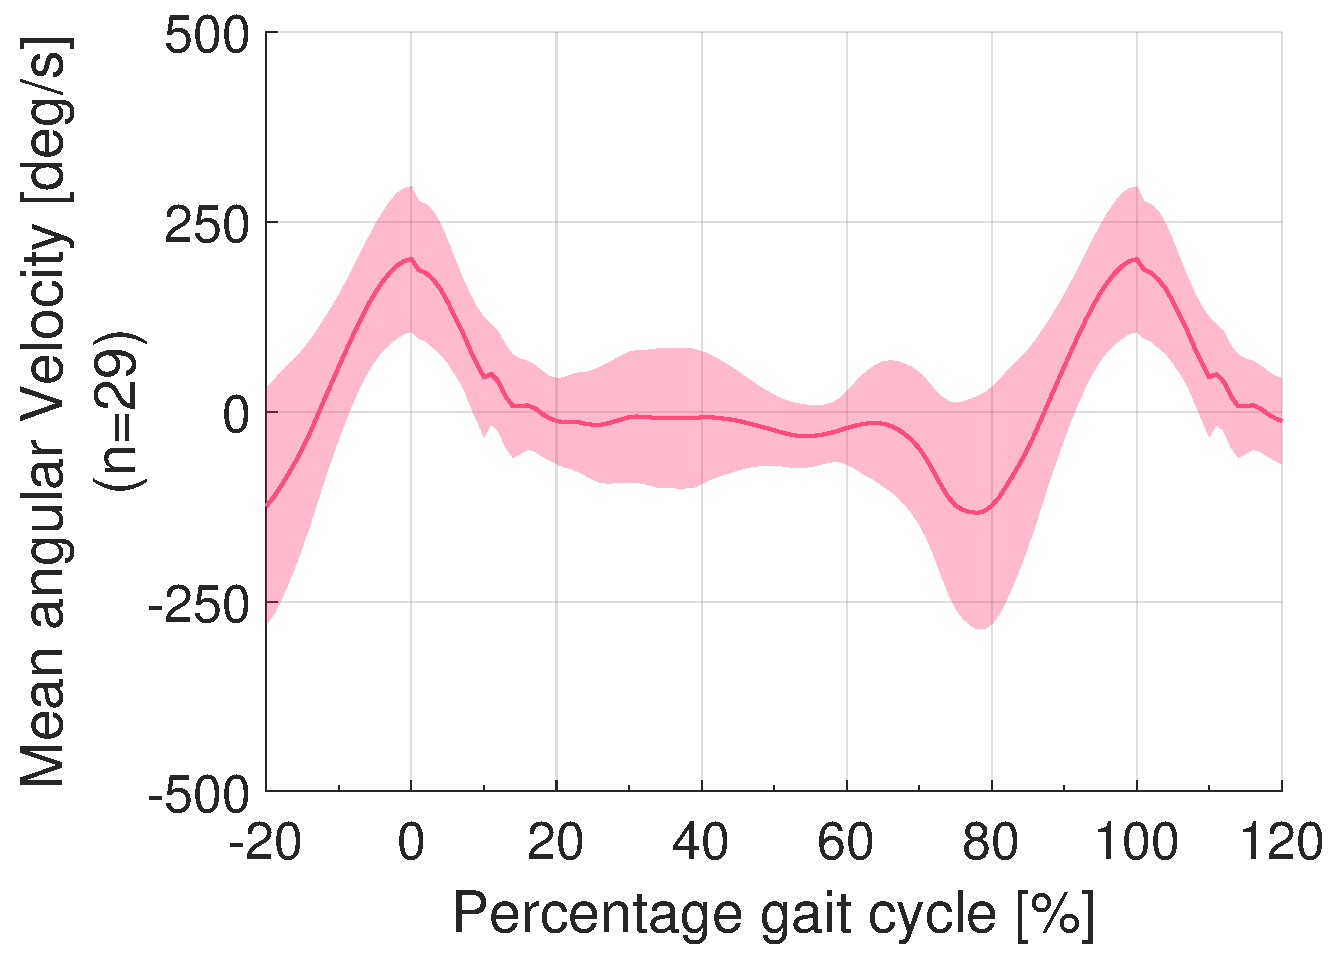
\includegraphics[width=0.275\linewidth]{content/6-Amputee/Gait-Trends/ch6_amputee_gait_trends_r_ankle_gyro_z_activity_stair_up.pdf} \\
        
        \rotatebox{90}{\quad \textbf{Stair Descent}} & 
        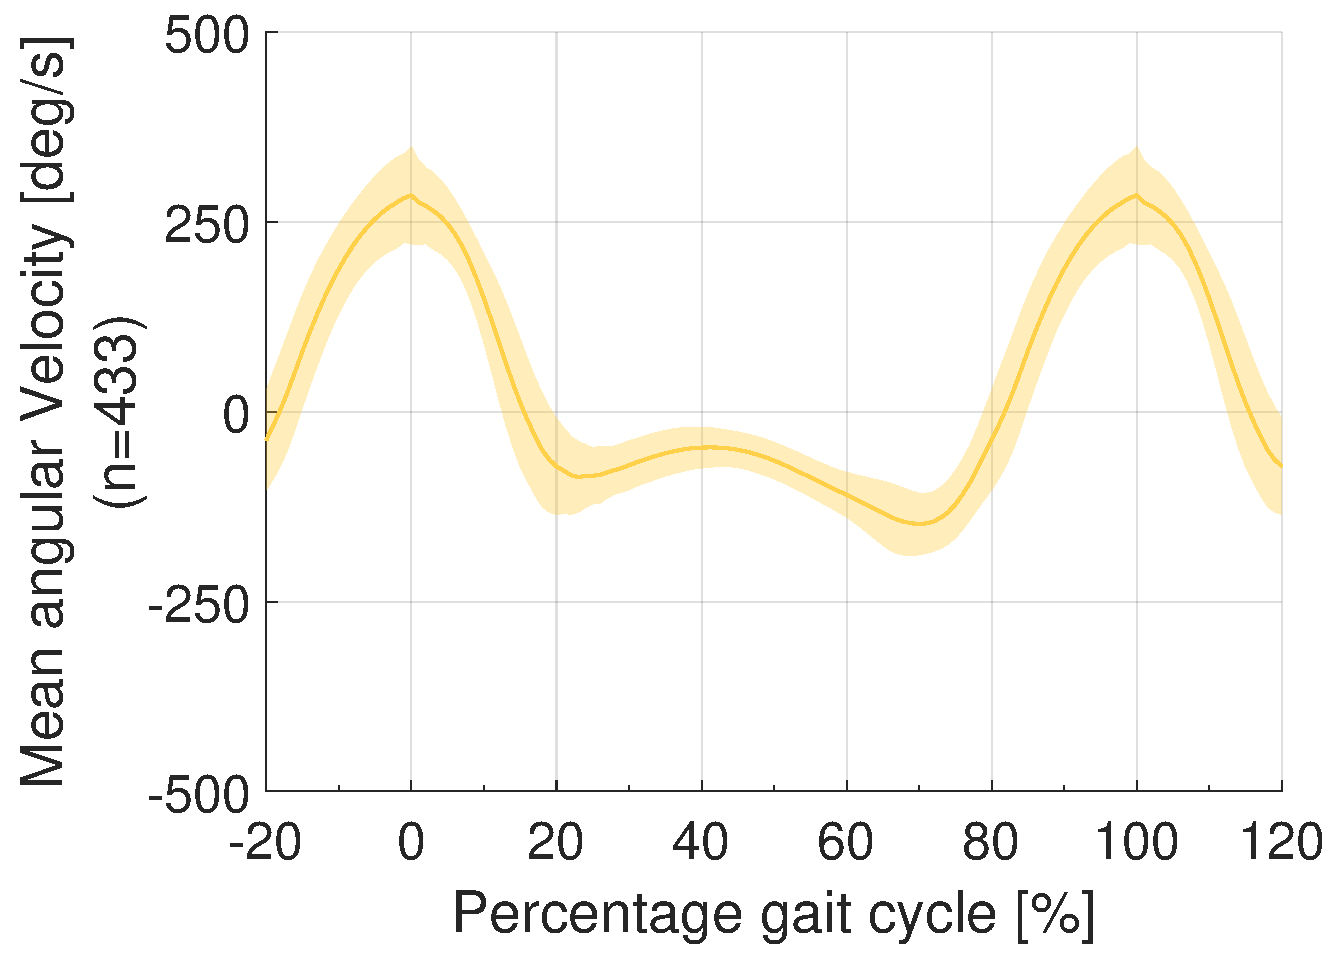
\includegraphics[width=0.275\linewidth]{content/6-Amputee/Gait-Trends/ch6_subject_01_gait_trends_r_ankle_gyro_z_activity_stair_down.pdf} & 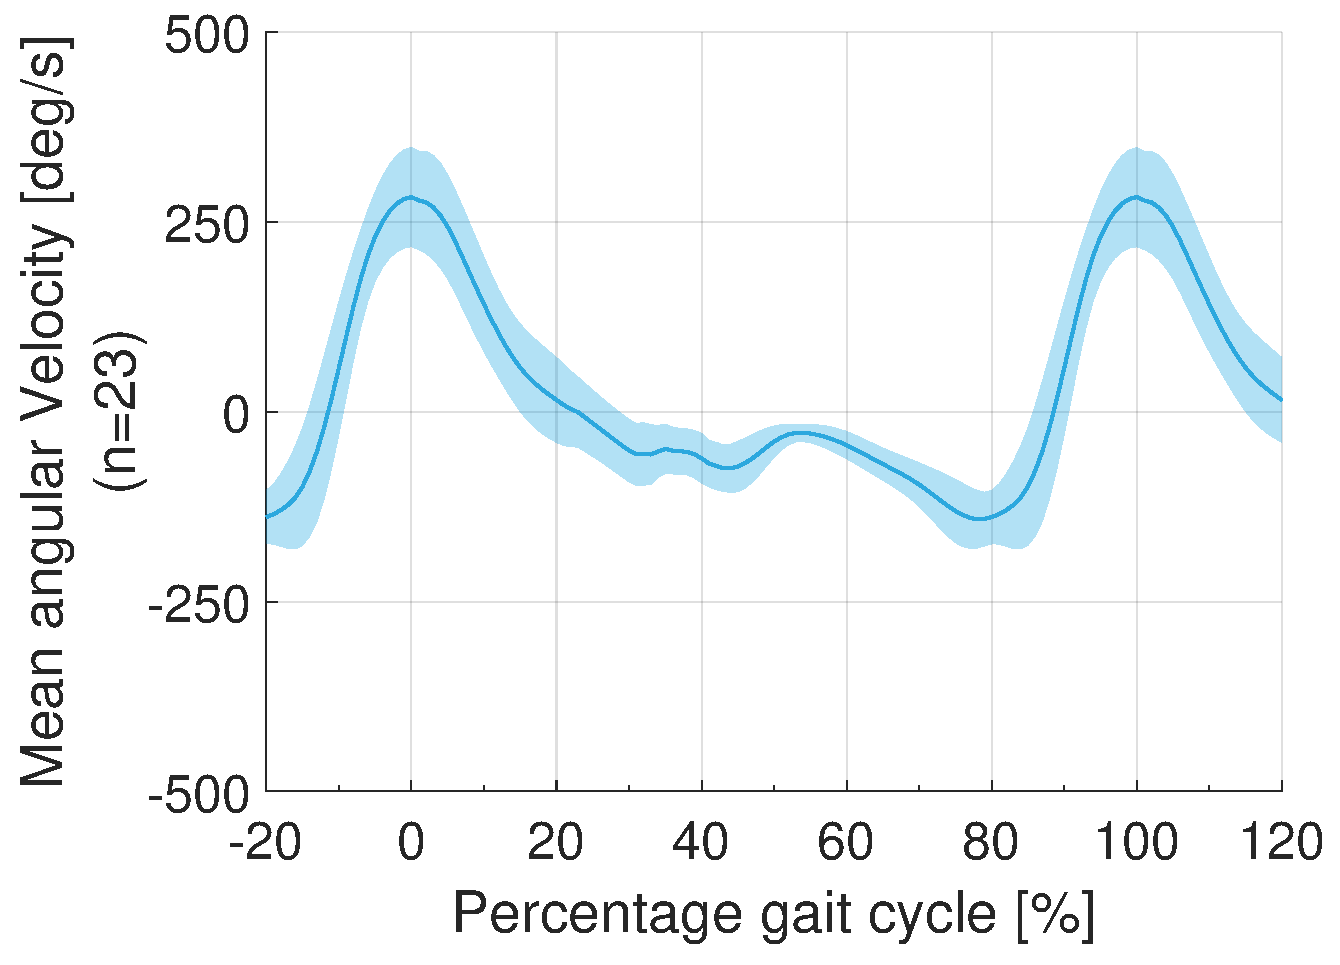
\includegraphics[width=0.275\linewidth]{content/6-Amputee/Gait-Trends/ch6_amputee_gait_trends_l_ankle_gyro_z_activity_stair_down.pdf} &
        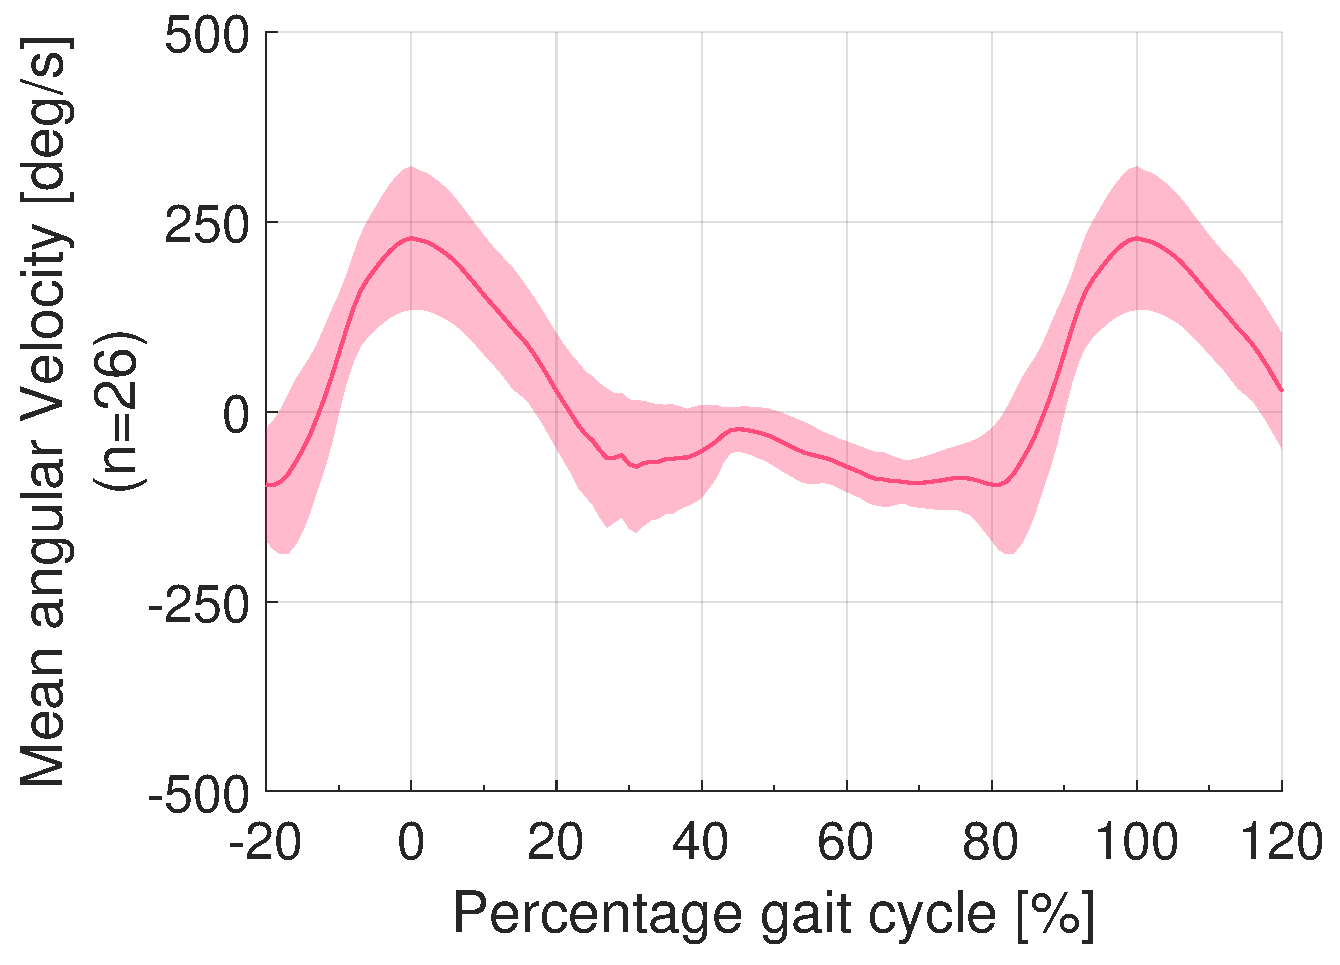
\includegraphics[width=0.275\linewidth]{content/6-Amputee/Gait-Trends/ch6_amputee_gait_trends_r_ankle_gyro_z_activity_stair_down.pdf} \\
    \end{tabular}
    \centering
    % \hspace*{1cm}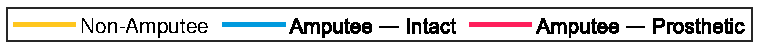
\includegraphics[width=0.7\textwidth]{content/6-Amputee/Gait-Trends/Legend.pdf}
    \caption[Angular velocity of the shank in the Saggital Plane for amputee and non-amputee during different activities.]{Angular velocity of the shank in the Saggital Plane for amputee and non-amputee during different activities. The yellow line is for Non-Amputee (Subject 01 Left Ankle); The blue line is the intact limb of  the trans-tibial amputee; The red line is the prosthetic of the trans-tibial amputee. The solid line shows the mean of the steps recorded for each activity. The filled area represents the standard deviation.}
    \label{fig:ch6_amputee_gyro_trends}
\end{figure}

From a visual assessment of plots difference between the intact and amputated limbs can be seen. On the prosthetic side changes in angular velocity are less smooth across all activities. This is particularly visible during early swing (approximately 80\% to 100\% gait cycle) where there is a kink in the upward velocity rise not seen in the intact limb. Changes in angular velocity around strike (approximately 20\%) are also more abrupt.

The intact limb and non amputee are closer but show clear difference during early stance (approximately 20\% to 40\%) with a much lower velocity seen in the intact limb.

This analysis just covers one axis of the gyroscope. Visible difference can also be seen in the other two gyroscope axes and accelerometer. As the intact limb is closer to the non-amputee it should be expected that it will perform more highly than the prosthetic side.

%-----------------------------------------------------------------
\section{Baseline}
\label{sec:amputee-baseline}
General model performance - Right Ankle (Intact limb) $74.2\%\pm9.4$, Left Ankle (Amputated Limb) - $55.3\$\pm9.6$ 

\begin{figure}[hbt]
    \centering
    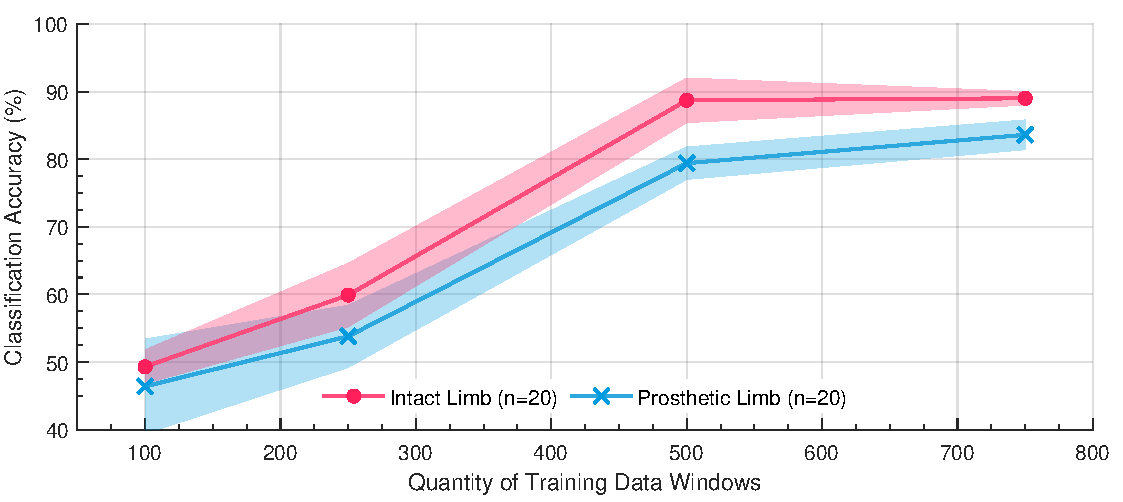
\includegraphics[width=\textwidth]{content/6-Amputee/ch6_baseline_model_accuracy.pdf}
    \caption[Classification accuracy for HAR model using increasing quantities of only amputee target data]{Classification accuracy for HAR model using increasing quantities of only amputee target data. The red line shows the performance of the trained model on the intact limb of a trans-tibial amputee. The blue line shows the performance of the trained model for the prosthetic side. The filled areas represent the standard deviation.}
    \label{fig:ch6-amputee-baseline-bespoke-model}
\end{figure}


%-----------------------------------------------------------------
\section{Data supplementation} % Are we going to include this?
\label{sec:amputee-supplementation}
\begin{table}[hbtp]
    \caption[Table of classification accuracy for amputee test data for a model trained using varying amounts of Source and Target training data]{Table of classification accuracy for amputee test data for a model trained using varying amounts of Source and Target training data. The cell value represents the percentage classification accuracy $\pm\sigma$ $(n=8)$. The highest classification accuracy for each quantity of target windows has been highlighted in bold}
    \label{tab:ch6-classfication-accuracy-mixed-source-target-right}
    \centering
    \begin{subtable}{\textwidth}
    \centering
    \caption{Intact Side} % Right
    \begin{tabularx}{0.99\textwidth}{cr| *{4}{Y}}
        \noalign{\hrule height 1.5pt}
        & & \multicolumn{4}{c}{\textbf{Target Training Windows}}\\
        & & 100 & 250 & 500 & 750 \\
        \hline
        \multirow{7}{*}{\rotatebox{90}{\parbox{3.4cm}{\centering\textbf{Source Training\\Windows}}}}
& 100 & $0.717{\scriptscriptstyle\pm0.03}$ & $0.682{\scriptscriptstyle\pm0.02}$ & $0.879{\scriptscriptstyle\pm0.02}$ & $0.877{\scriptscriptstyle\pm0.04}$ \\
& 250 & $0.764{\scriptscriptstyle\pm0.04}$ & $0.730{\scriptscriptstyle\pm0.03}$ & $0.883{\scriptscriptstyle\pm0.03}$ & $\mathbf{0.889{\scriptscriptstyle\pm0.01}}$ \\
& 500 & $0.800{\scriptscriptstyle\pm0.04}$ & $0.795{\scriptscriptstyle\pm0.03}$ & $0.875{\scriptscriptstyle\pm0.02}$ & $0.888{\scriptscriptstyle\pm0.02}$ \\
& 750 & $0.815{\scriptscriptstyle\pm0.01}$ & $0.801{\scriptscriptstyle\pm0.02}$ & $0.873{\scriptscriptstyle\pm0.02}$ & $0.881{\scriptscriptstyle\pm0.02}$ \\
& 1000 & $0.801{\scriptscriptstyle\pm0.04}$ & $0.786{\scriptscriptstyle\pm0.03}$ & $\mathbf{0.886{\scriptscriptstyle\pm0.03}}$ & $0.874{\scriptscriptstyle\pm0.02}$ \\
& 1500 & $\mathbf{0.835{\scriptscriptstyle\pm0.03}}$ & $0.794{\scriptscriptstyle\pm0.06}$ & $0.871{\scriptscriptstyle\pm0.01}$ & $0.875{\scriptscriptstyle\pm0.03}$ \\
& 3000 & $0.825{\scriptscriptstyle\pm0.01}$ & $\mathbf{0.826{\scriptscriptstyle\pm0.07}}$ & $0.846{\scriptscriptstyle\pm0.03}$ & $0.863{\scriptscriptstyle\pm0.03}$ \\
        \noalign{\hrule height 1.5pt}\\
        \end{tabularx}
    \end{subtable}
    
    \begin{subtable}{\textwidth}
    \centering
    \caption{Prostheses Side} % Left
    \begin{tabularx}{0.99\textwidth}{cr| *{4}{Y}}
        \noalign{\hrule height 1.5pt}
        & & \multicolumn{4}{c}{\textbf{Target Training Windows}}\\
        & & 100 & 250 & 500 & 750 \\
        \hline
        \multirow{7}{*}{\rotatebox{90}{\parbox{3.4cm}{\centering\textbf{Source Training\\Windows}}}}
& 100 & $0.626{\scriptscriptstyle\pm0.05}$ & $0.643{\scriptscriptstyle\pm0.03}$ & $0.855{\scriptscriptstyle\pm0.02}$ & $0.813{\scriptscriptstyle\pm0.04}$ \\
& 250 & $0.714{\scriptscriptstyle\pm0.04}$ & $0.611{\scriptscriptstyle\pm0.02}$ & $0.836{\scriptscriptstyle\pm0.05}$ & $0.843{\scriptscriptstyle\pm0.03}$ \\
& 500 & $0.752{\scriptscriptstyle\pm0.03}$ & $0.729{\scriptscriptstyle\pm0.08}$ & $0.842{\scriptscriptstyle\pm0.02}$ & $0.840{\scriptscriptstyle\pm0.05}$ \\
& 750 & $0.734{\scriptscriptstyle\pm0.06}$ & $0.712{\scriptscriptstyle\pm0.04}$ & $0.848{\scriptscriptstyle\pm0.03}$ & $0.847{\scriptscriptstyle\pm0.02}$ \\
& 1000 & $0.756{\scriptscriptstyle\pm0.02}$ & $0.756{\scriptscriptstyle\pm0.08}$ & $\mathbf{0.875{\scriptscriptstyle\pm0.03}}$ & $\mathbf{0.872{\scriptscriptstyle\pm0.01}}$ \\
& 1500 & $0.734{\scriptscriptstyle\pm0.02}$ & $\mathbf{0.764{\scriptscriptstyle\pm0.05}}$ & $0.869{\scriptscriptstyle\pm0.02}$ & $0.852{\scriptscriptstyle\pm0.02}$ \\
& 3000 & $\mathbf{0.767{\scriptscriptstyle\pm0.02}}$ & $\mathbf{0.764{\scriptscriptstyle\pm0.04}}$ & $0.874{\scriptscriptstyle\pm0.02}$ & $0.849{\scriptscriptstyle\pm0.02}$ \\
        \noalign{\hrule height 1.5pt}\\
    \end{tabularx}
    \end{subtable}
\end{table}


%-----------------------------------------------------------------
\section{Transfer Learning}
\label{sec:amputee-transfer}
\begin{figure}[hbtp]
    \centering
    \begin{subfigure}{\textwidth}
        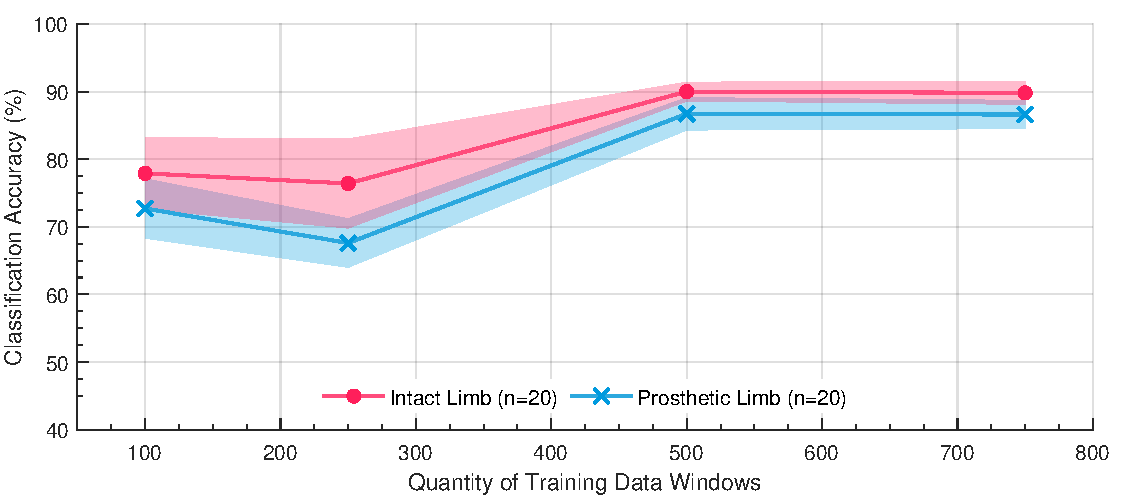
\includegraphics[width=\textwidth]{content/6-Amputee/ch6_pre_trained_model_accuracy.pdf}
        \caption{Fine tuning all layers}
    \end{subfigure}
    \begin{subfigure}{\textwidth}
        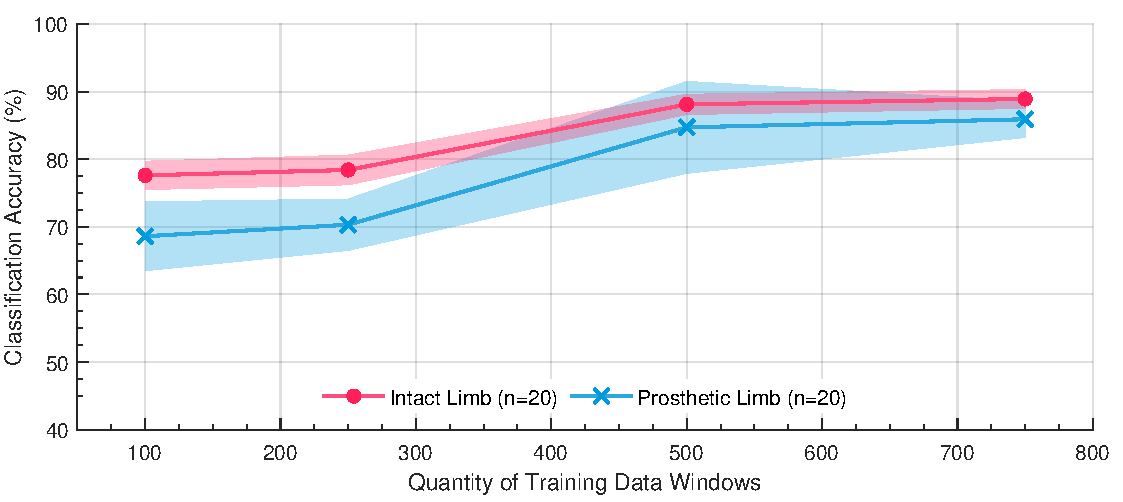
\includegraphics[width=\textwidth]{content/6-Amputee/ch6_frozen_lstm_layer_accuracy.pdf}
        \caption{Fine tuning only the dense layer}
    \end{subfigure}
    \caption[Classification accuracy for re-training a pre-trained model using increasing quantities of amputee target data]{Classification accuracy for re-training a pre-trained model using increasing quantities of amputee target data. The red line shows the performance of the trained model on the intact limb of a trans-tibial amputee. The blue line shows the performance of the trained model for the prosthetic side. The filled areas represent the standard deviation.}
    \label{fig:ch6-amputee-retrain-pre-trained}
\end{figure}
\begin{figure}[t]\ContinuedFloat
    \centering
    \begin{subfigure}{\textwidth}
        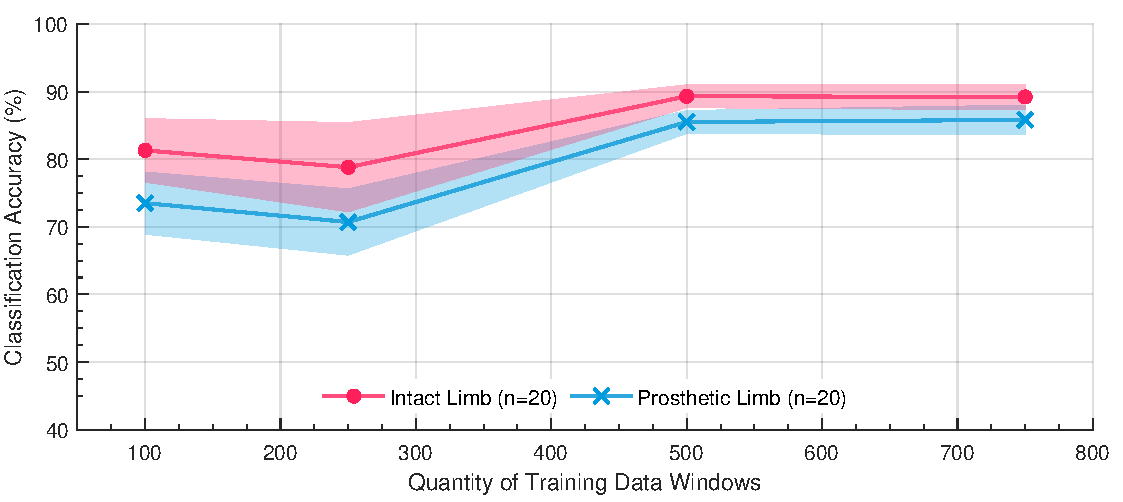
\includegraphics[width=\textwidth]{content/6-Amputee/ch6_frozen_dense_layer_accuracy.pdf}
        \caption{Fine tuning only the \acrshort{lstm} layer}
    \end{subfigure}
    \caption[]{Classification accuracy for re-training a pre-trained model using increasing quantities of amputee target data (Cont.).}
\end{figure}


%-----------------------------------------------------------------
\section{Discussion}
\label{sec:amputee-discussion}
What were we trying to achieve and have we achieved it?

Any interesting observations?
% Does this work act like the non-amputee?

Do any of the methods show promise?


What are the limitations of this study/methods?
%Very limited amounts of data

Areas for further work/improvements?
%Ensemble methods?
%-----------------------------------------------------------------
\section{Conclusions}
\label{sec:amputee-conclusions}
What were the research aims?

Have we met the research aims/outcomes of this work?

What are we going to do next?